\documentclass{article}
\usepackage{header} % Required for inserting images
% \newcommand{\p}[1]{$\mathbb{P}(#1)$}


\title{\LARGE{Теория вероятностей и математическая статистика—2}\\
Теоретический и задачный минимумы\\
ФЭН НИУ ВШЭ}
\author{Винер Даниил  \href{https://t.me/danya_vin}{@danya\_vin}}
\date{Версия от \today}

\begin{document}
\maketitle
\tableofcontents
\newpage
\setlength{\parindent}{15pt}
\setlength{\parskip}{2mm}
\setlist[itemize]{left=1cm}
\setlist[enumerate]{left=1cm}
\section{Теоретический минимум}
% \comment Обозначение $\exp\left(\text{equation}\right)$ равносильно $e^{\text{equation}}$

\subsection{Дайте определение нормально распределённой случайной величины. Для неё укажите диапазон возможных значений, функцию плотности, ожидание, дисперсию. Нарисуйте функцию плотности}
\definition Случайная величина имеет нормальное распределение $X\sim\mathcal{N}(\mu,\sigma^2)$, если функция плотности равна
\begin{equation*}
    f_X(x)=\frac{1}{\sigma\sqrt{2\pi}}\exp\left(-\frac{1}{2}\left(\frac{x-\mu}{\sigma}\right)^2\right)
\end{equation*}
\begin{itemize}
    \item Случайная величина $X\sim\mathcal{N}(\mu,\sigma^2)$ принимает любые значения $(-\infty,+\infty)$
    \item $\matwait{X}=\mu$
    \item $\dispersia{X}=\sigma^2$
\end{itemize}
% 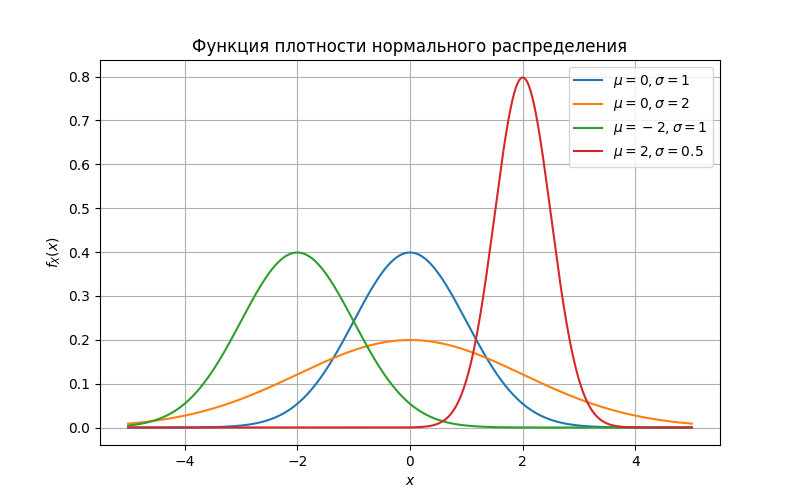
\includegraphics[width=0.7\linewidth]{normal.png}
\begin{figure}[h]
    \centering
    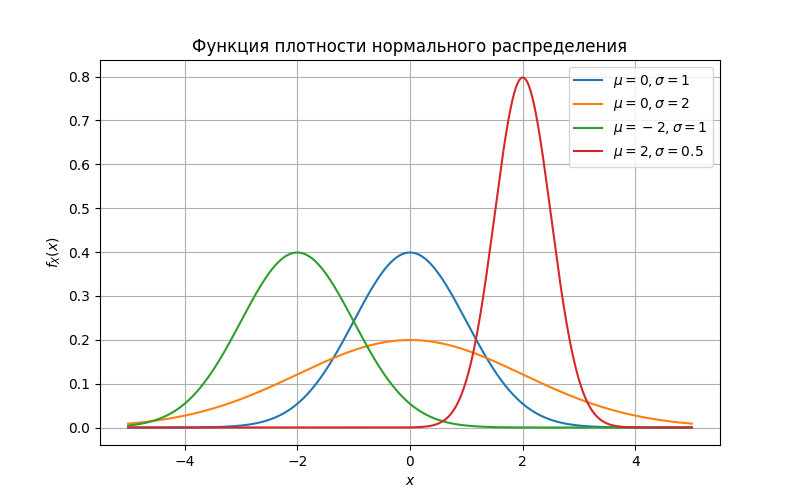
\includegraphics[width=0.8\linewidth]{normal.png}
\end{figure}


\newpage
\subsection{С помощью нормальных случайных величин дайте определение случайной величины, имеющей хи-квадрат распределение. Для хи-квадрат распределённой случайной величины укажите диапазон возможных значений, математическое ожидание и дисперсию. Нарисуйте функцию плотности при разных степенях свободы}
\definition Случайная величина $X$ имеет $\chi^2$-распределение с $m$ степенями свободы, $H\sim\chi^2(m)$, если $X$ представима в виде
\begin{equation*}
    X=X_1^2+\ldots+X_m^2,
\end{equation*}
где $X_1,\ldots,X_m\sim iidN(0,1)$ (independent identically distributed normal — независимые одинаково распределенные нормально распределенные случайные величины)
\begin{itemize}
    \item Принимает значения $x\in[0;+\infty]$
    \item $\matwait{X}=m$
    \item $\dispersia{X}=2m$
\end{itemize}
\begin{figure}[h]
    \centering
    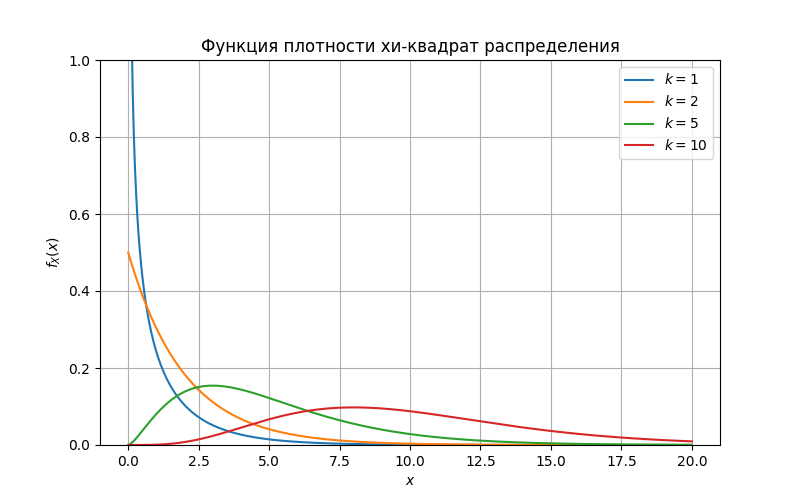
\includegraphics[width=0.8\linewidth]{chi.png}
\end{figure}

\newpage
\subsection{С помощью нормальных случайных величин дайте определение случайной величины, имеющей распределения Стьюдента. Для случайной величины, распределённой по Стьюденту, укажите диапазон возможных значений. Нарисуйте функцию плотности распределения Стьюдента при разных степенях свободы на фоне нормальной стандартной функции плотности.}
\definition Пусть $\xi_0, \xi_1, \ldots, \xi_k$ независимы и имеют стандартное нормальное распределение. Распределение случайной величины
$$
t_k=\frac{\xi_0}{\sqrt{\frac{\xi_1^2+\ldots+\xi_k^2}{k}}}
$$
называется распределением Стьюдента с $k$ степенями свободы и обозначается $\mathrm{T}_k$.

Распределение Стьюдента совпадает с распределением случайной величины $t_k=\frac{\xi}{\sqrt{\chi_k^2 / k}}$, где $\xi \in \mathcal{N}(0,1)$ и $\chi_k^2 \in \mathrm{H}_k$ независимы.
\begin{itemize}
    \item Принимает значения в диапазоне $(-\infty;+\infty)$
    \item $\matwait{t_k}=0$ при $k>1$, а при $k=1$ матожидание не существует, так как интеграл расходится (распределение Коши)
    \item $\dispersia{t_k}=\displaystyle\frac{k}{k-2}$, $\exists$ только при $k>2$
\end{itemize}

\begin{figure}[h]
    \centering
    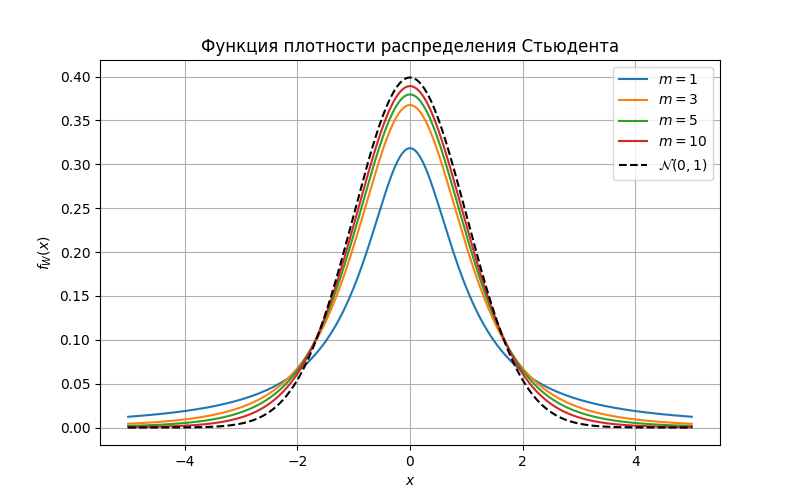
\includegraphics[width=0.8\linewidth]{student.png}
\end{figure}


\newpage
\subsection{С помощью нормальных случайных величин дайте определение случайной величины, имеющей распределение Фишера. Для случайной величины, распределённой по Фишеру, укажите диапазон возможных значений. Нарисуйте возможную функцию плотности}
\definition Случайная величина $F\sim F(k,m)$ имеет распределение Фишера с параметрами $k$ и $m$ (степени свободы), если она может быть представлена в виде:
\begin{equation*}
    F = \frac{X_k/k}{X_m/m}
\end{equation*}
где $X_k\sim\chi^2(k),\ X_m\sim\chi^2(m)$ и $X_k,\ X_m$ — независимы

\begin{itemize}
    \item $F$ принимает значения из диапазона $[0;+\infty]$
\end{itemize}

\begin{figure}[h]
    \centering
    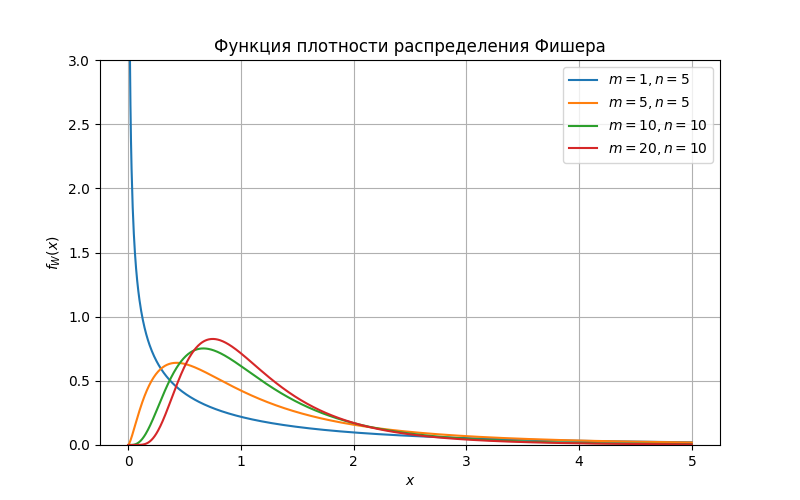
\includegraphics[width=0.8\linewidth]{fisher.png}
\end{figure}

\subsection{Дайте определение выборочного среднего и выборочной дисперсии}
\definition Выборочное среднее — $\overline{X}:=\displaystyle\frac{X_1+\ldots+X_n}{n}$

\definition Неисправленная выборочная дисперсия — $s^2:=\displaystyle\frac{1}{n}\sum_{i=1}^n (X_i-\overline{X})^2$

\definition Исправленная выборочная дисперсия — $\widehat{\sigma}^2:=\displaystyle\frac{1}{n-1}\sum_{i=1}^n (X_i-\overline{X})^2$


\subsection{Дайте определение выборочного начального и выборочного центрального момента порядка $k$}
Пусть дана выборка $X=(X_1,\ldots,X_n)$

\definition Выборочным \textit{начальным} моментом порядка $k$ называется число 
\begin{equation*}
    \frac{1}{n}\sum_{i=1}^{k}(X_i)^k
\end{equation*}

\definition Выборочным \textit{центральным} моментом порядка $k$ называется число
\begin{equation*}
    \frac{1}{n}\sum_{i=1}^{k}(X_i-\overline{X})^k
\end{equation*}



\subsection{Дайте определение выборочной функции распределения}
\definition Выборочная (эмпирическая) функция распределения — это $$\hat{F}_n(x)=\frac{1}{n}\sum_{i=1}^{n}I\{X_i\leqslant x\},$$ где $I\{X_i\leqslant x\}$ — индикаторная функция, равная 1, если $X_i\leqslant x$, и 0 в противном случае

% \definition Выборочной функцией распределения называется \begin{equation*}
%     \begin{aligned}
%         \hat{F_n}(x)&=\displaystyle\frac{\text{число элементов случайной выборки, которые нестрого меньше } x}{n}\\
%         &=\frac{\#\{i\in\{1,\ldots,n\}:\ X_i\leqslant x\}}{n}
%         % &=\frac{1}{n}\sum_{i=1}^n 
%     \end{aligned}
% \end{equation*}

\subsection{Выпишите формулу несмещённой оценки дисперсии}
\definition $\widehat{\sigma}^2:=\displaystyle\frac{1}{n-1}\sum_{i=1}^n (X_i-\overline{X})^2$


\subsection{Дайте определение несмещённой оценки $\widehat{\theta}$ параметра $\theta$}
\definition Оценка $\hat{\theta}$ неизвестного параметра $\theta\in\Theta$ называется \textit{несмещённой}, если 
\begin{equation*}
    \matwait{\hat{\theta}}=\theta\ \forall\theta\in\Theta,
\end{equation*}
где $\Theta$ — множество всех параметров $\theta$

\subsection{Дайте определение состоятельной последовательности оценок $\widehat{\theta}_n$; Укажите условия на $\matwait{\widehat{\theta}_n}$ и $\dispersia{\widehat{\theta}_n}$, достаточные для состоятельности}
\definition Последовательность оценок $\hat{\theta}_n$ называется \textit{состоятельной оценкой} неизвестного параметра $\theta\in\Theta$, если
\begin{equation*}
    \forall \theta\in\Theta\ \hat{\theta}_n\underset{n\to\infty}{\overset{\mathbb{P}}{\longrightarrow}}\theta,
\end{equation*}
то есть $\hat{\theta}_n$ сходится по вероятности к $\theta$
\begin{equation*}
    \forall\varepsilon>0:\ \lim\limits_{n\to\infty}\mathbb{P}(|\hat{\theta}_n-\theta|\geqslant\varepsilon)=0
\end{equation*}

\theorem Если оценка асимптотически несмещенная и её дисперсия стремится к нулю, то такая оценка будет состоятельной. То есть должны выполняться такие условия:
\begin{itemize}
    \item Асимптотическая несмещённость — $\lim\limits_{n\to\infty}\matwait{\widehat{\theta}_n}=\theta$
    \item Сходимость дисперсии к нулю — $\lim\limits_{n\to\infty}\dispersia{\widehat{\theta}_n}=0$
\end{itemize}




\subsection{Дайте определение эффективности оценки $\widehat{\theta}$ среди множества оценок $\widehat{\Theta}_n$}
\definition Оценка $\hat{\Theta}$ называется эффективной в классе $K$, если $\forall\ \widetilde{\Theta}\in K$
\begin{equation*}
    \begin{aligned}
        \matwait{\hat{\Theta}-\Theta}^2&\leqslant\matwait{\widetilde{\Theta}-\Theta}^2\text{причем }\exists \Theta_0:\\
        \matwait{\hat{\Theta}-\Theta_0}^2&<\matwait{\widetilde{\Theta}-\Theta_0}^2
    \end{aligned}
\end{equation*}
Класс $K$ обладает смещением $b(\Theta)$

\definition Оценка $\hat{\Theta}$ называется эффективной в классе несмещенных оценок, если $\forall\ \widetilde{\Theta}\in K$
\begin{equation*}
    \begin{aligned}
        \dispersia{\hat{\Theta}}&\leqslant \dispersia{\widetilde{\Theta}},\text{причем }\exists \Theta_0:\\
        \dispersia{\hat{\Theta}}&< \dispersia{\widetilde{\Theta}}\text{для }\Theta_0
    \end{aligned}
\end{equation*}



\newpage
\section{Задачный минимум}
\subsection{Для взрослого мужчины рост в сантиметрах, величина $X$, и вес в килограммах, величина $Y$...}
$X$ — рост, $Y$ — вес, $Z=(X,Y)$, $\matwait{Z}=\begin{pmatrix}
    175\\
    74
\end{pmatrix}$, $V(Z)=\begin{pmatrix}
    49&28\\
    28&36
\end{pmatrix}$
\subsubsection*{a)}
\textbf{Вариант 1.} Найдем вероятность противоположного события:
\begin{equation*}
    \begin{aligned}
        \prob{|X-\matwait{X}|\leqslant 10}&=\prob{-10\leqslant X-175\leqslant 10}\\
        &\text{проведем стандартизацию и нормализацию}\\
        &=\mathbb{P}\left(\left\{\frac{-10}{7}\leqslant \frac{X-175}{7}\leqslant \frac{10}{7}\right\}\right)\\
        &=\Phi\left(\frac{10}{7}\right)-\Phi\left(-\frac{10}{7}\right)\\
        &=2\Phi\left(\frac{10}{7}\right)-1\\
        &\approx0.1531
    \end{aligned}
\end{equation*}

\textbf{Вариант 2.} Найдем вероятность непосредственно искомого события
\begin{equation*}
    \begin{aligned}
        \prob{|X-\matwait{X}|>10}&=\mathbb{P}\left(\left|\frac{X-175}{\sqrt{49}}\right|>\frac{10}{\sqrt{49}}\right)\\
        &\text{пусть }\left|\frac{X-175}{\sqrt{49}}\right|=|Z|\\
        &=2\cdot\left(1-\mathbb{P}\left(Z\leqslant\frac{10}{\sqrt{49}}\right)\right)\\
        &\approx0.153
    \end{aligned}
\end{equation*}

\subsubsection*{б)}
Так как $Z$ имеет многомерное нормальное распределение, то $U$ также имеет нормальное распределение
\begin{equation*}
    \begin{aligned}
        \matwait{U}&=\matwait{X}-\matwait{Y}\\
        &=175-74\\
        &=101\\
        \dispersia{U}&=\dispersia{X}+\dispersia{Y}-2cov(X,Y)\\
        &=49+46-2\cdot28\\
        &=29
    \end{aligned}
\end{equation*}

Стандартная функция плотности нормального распределения:
\begin{equation*}
    \begin{aligned}
        f_X(x)=\frac{1}{\sqrt{2\pi\sigma^2}}\exp\left(-\frac{(x-\mu)^2}{2\sigma^2}\right)
    \end{aligned}
\end{equation*}
Тогда, в нашем случае:
\begin{equation*}
    f_U(u)=\frac{1}{\sqrt{2\pi 29}}\exp\left(-\frac{(u-101)^2}{2\cdot29}\right)
\end{equation*}


\subsubsection*{в)}
\begin{equation*}
    \begin{aligned}
        \prob{U<90}&=\mathbb{P}\left(\left\{\frac{U-101}{\sqrt{29}}<\frac{90-101}{\sqrt{29}}\right\}\right)\\
        &=\Phi(-2.0426)\\
        &\approx0.0205
    \end{aligned}
\end{equation*}


\subsection{Рост в сантиметрах, случайная величина $X$, и вес в килограммах, случайная величина $Y$...}
\theorem Если $(X,Y)\sim N\left(\begin{pmatrix}
    \mu x\\
    \mu y
\end{pmatrix}, \begin{pmatrix}
    \sigma_x^2&\rho\sigma_x\sigma_y\\
    \rho\sigma_y\sigma_x&\sigma_y^2
\end{pmatrix}\right)$, где $\rho=\displaystyle\frac{cov(X,Y)}{\sigma_X\sigma_Y}$ — коэффициент корреляции, то 
\begin{equation*}
    \begin{aligned}
        (X|Y=y)&\sim N\left(\mu_x+\rho\frac{\sigma_x}{\sigma_y}(y-\mu_y),\ \sigma_x^2\left(1-\rho^2\right)\right)\\
        (Y|X=x)&\sim N\left(\mu_y+\rho\frac{\sigma_y}{\sigma_x}(x-\mu_x),\ \sigma_y^2\left(1-\rho^2\right)\right)
    \end{aligned}
\end{equation*}

\subsubsection*{a)}
% $\matwait{Y|X=170}$
$\rho=\displaystyle\frac{cov(X,Y)}{\sigma_X\sigma_Y}=\frac{28}{\sqrt{49\cdot36}}=\frac{2}{3}$

\begin{equation*}
    \begin{aligned}
        % (Y|X=170)&\sim N
        (Y|X=170)&\sim N\left(\underbrace{74+\frac{2}{3}\cdot\frac{6}{7}\cdot(170-175)}_{\matwait{Y|X=170}=71.14};\ \underbrace{36\left(1-\frac{4}{9}\right)}_{\dispersia{Y|X=170}}\right)\\
        (Y|X=170)&\sim N\left(71.1;20\right)
    \end{aligned}
\end{equation*}

\subsubsection*{б)}
\begin{equation*}
    \begin{aligned}
        f_{Y|X=170}(a)=\frac{1}{\sqrt{2\pi20}}\exp\left(-\frac{(a-71.14)^2}{2\cdot20}\right)
    \end{aligned}
\end{equation*}


\subsubsection*{в)}

\begin{equation*}
    \begin{aligned}
        \prob{Y>90|X=170}&=\mathbb{P}\left(\left\{\frac{Y-71.14}{\sqrt{20}}>\frac{90-71.14}{\sqrt{20}}\right\}\right)\\
        &=1-\mathbb{P}\left(\left\{\frac{Y-71.14}{\sqrt{20}}\leqslant\frac{90-71.14}{\sqrt{20}}\right\}\right)
    \end{aligned}
\end{equation*}



% \begin{equation*}
%     \begin{aligned}
%         \prob{Y>90|X=170}&=\prob{\left.\frac{Y-71.14}{\sqrt{20}}>\frac{90-71.14}{\sqrt{20}}\right|X=170}\\
%         &=1-\prob{\left.\frac{Y-71.14}{\sqrt{20}}<4.217\right|X=170}\\
%         &\approx 0.000013\\
%         &\approx0
%     \end{aligned}
% \end{equation*}



\subsection{Для реализации случайной выборки $x = (1, 0,-1, 1)$ найдите...}
% \subsubsection*{a)} 
\begin{itemize}
    \item[\textbf{a)}] выборочное среднее
    \begin{equation*}
        \overline{X}=\displaystyle\frac{X_1+\ldots+X_n}{n}=\frac{1+0-1+1}{4}=\frac{1}{4}
    \end{equation*}

    \item[\textbf{b)}] неисправленную выборочную дисперсию
    \begin{equation*}
        \begin{aligned}
            s^2&=\frac{1}{n}\sum_{i=1}^n\left(X_i-\overline{X}\right)^2\\
            &=\frac{1}{4}\left(\left(1-\frac{1}{4}\right)^2+\left(0-\frac{1}{4}\right)^2+\left(-1-\frac{1}{4}\right)^2+\left(1-\frac{1}{4}\right)^2\right)\\
            % &=\frac{11}{16}\\
            &\approx0.68
        \end{aligned}
    \end{equation*}

    \item[\textbf{c)}] исправленную выборочную дисперсию
    \begin{equation*}
        \begin{aligned}
            \widehat{\sigma}^2&=\frac{1}{n-1}\sum_{i=1}^n\left(X_i-\overline{X}\right)^2=\frac{n}{n-1}s^2\\
            &\approx0.91
        \end{aligned}
    \end{equation*} 

    \item[\textbf{d)}] выборочный второй начальный момент
    
    Выборочный $k$-й начальный момент = $\displaystyle\frac{1}{n}\sum_{i=1}^n\left(X_i\right)^k$

    В нашем случае:
    \begin{equation*}
        \frac{1}{4}\left(1^2+0^2+(-1)^2+1^2\right)=\frac{3}{4}
    \end{equation*}
    
    \item[\textbf{e)}] выборочный третий центральный момент
    
    Выборочный $k$-й центральный момент = $\displaystyle\frac{1}{n}\sum_{i=1}^n\left(X_i-\overline{X}\right)^k$

    В нашем случае:
    \begin{equation*}
        \frac{1}{4}\left(\left(1-\frac{1}{4}\right)^3+\left(0-\frac{1}{4}\right)^3+\left(-1-\frac{1}{4}\right)^3+\left(1-\frac{1}{4}\right)^3\right)=-\frac{9}{32}\approx-0.28
    \end{equation*}
    % \begin{equation*}
    %     \begin{aligned}
    %         ans=&\frac{1}{4}\left(\left(1-\frac{1}{4}\right)^3+\left(0-\frac{1}{4}\right)^3+\left(-1-\frac{1}{4}\right)^3+\left(1-\frac{1}{4}\right)^3\right)\\
    %         &=\frac{1}{3}
    %     \end{aligned}
    % \end{equation*}
\end{itemize}


\subsection{Для реализации случайной выборки $x = (1, 0,-1, 1)$ найдите...}
\begin{itemize}
    \item[\textbf{a)}] вариационный ряд 
    \begin{equation*}
        \begin{aligned}
            X&=sort(list(X_1,\ldots,X_n))\\%\footnote[1]{эту строчку можно не писать}\\
            &=(-1,0,1,1)
        \end{aligned}
    \end{equation*}

    \item[\textbf{b)}] первый член вариационного ряда — $-1$
    \item[\textbf{c)}] последний член вариационного ряда — $1$ 
    \item[\textbf{d)}] график выборочной функции распределения
    
    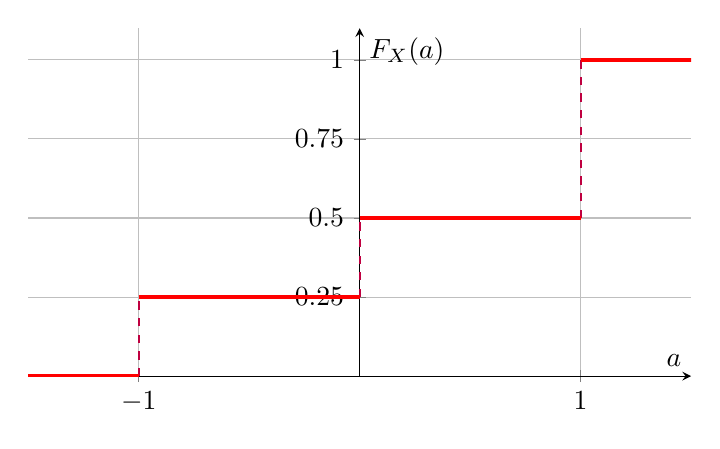
\begin{tikzpicture}
        \begin{axis}[
            width=10cm, height=6cm,
            axis x line=middle, axis y line=middle,
            xtick={-1,0,1}, ytick={0,0.25,0.5,0.75,1},
            ymin=0, ymax=1.1, xmin=-1.5, xmax=1.5,
            xlabel={$a$}, ylabel={$F_X(a)$},
            samples=100, domain=-2:2,
            grid=major
        ]
            % Пунктирные вертикальные линии
            \addplot[dashed, purple, thick] coordinates {(-1,0) (-1,0.25)};
            \addplot[dashed, purple, thick] coordinates {(0,0.25) (0,0.5)};
            \addplot[dashed, purple, thick] coordinates {(1,0.5) (1,1)};
            
            % Жирные красные горизонтальные линии
            \addplot[red, very thick] coordinates {(-1,0.25) (0,0.25)};
            \addplot[red, very thick] coordinates {(0,0.5) (1,0.5)};
            
            % Горизонтальная линия слева (-\infty до -1)
            \addplot[red, very thick] coordinates {(-2,0) (-1,0)};
            
            % Горизонтальная линия справа (от 1 до +\infty)
            \addplot[red, very thick] coordinates {(1,1) (2,1)};
        \end{axis}
    \end{tikzpicture}
\end{itemize}

\subsection{Пусть $X_1,\ldots, X_n$ — случайная выборка из дискретного распределения, заданного с помощью таблицы}
\begin{equation*}
    \begin{tabular}{cccc}
        \hline
        $x$ & $-3$ & $0$ & $2$\\
        \hline
        $\mathbb{P}(X_i=x)$ & $2/3-\theta$ & 1/3 & $\theta$\\
        \hline
    \end{tabular}
\end{equation*}

Рассмотрите оценку $\widehat{\theta}=\displaystyle\frac{\overline{X}+2}{5}$
\begin{itemize}
    \item[\textbf{a)}] \begin{equation*}
        \begin{aligned}
            \matwait{\widehat{\theta}}&=\matwait{\frac{\overline{X}+2}{5}}\\
            &=\frac{1}{5}\left(\overline{X}+2\right)\\
            &=\frac{1}{5}\left((-3)\cdot\left(\frac{2}{3}-\theta\right)+0\cdot\frac{1}{3}+2\theta+2\right)\\
            &=\theta
        \end{aligned}
    \end{equation*}

    \item[\textbf{b)}] Является ли оценка $\widehat{\theta}$ несмещённой оценкой неизвестного параметра $\theta$?
    
    Да, так как $\matwait{\widehat{\theta}}=\theta\ \forall\theta\in\Theta$ по доказанному в пункте \textbf{a)}
\end{itemize}

\subsection{Пусть $X_1,\ldots, X_n$ — случайная выборка из распределения с плотностью распределения}
\begin{equation*}
    f(x,\theta)=\begin{cases}
        \frac{6x(\theta-x)}{\theta^3},&\text{ при }x\in[0;\theta]\\
        0,&\text{ при }x\notin[0;\theta],
    \end{cases}
\end{equation*}
где $\theta>0$ — неизвестный параметр распределения и $\hat{\theta}=\overline{X}$

\begin{itemize}
    \item[\textbf{a)}] Является ли оценка $\widehat{\theta}=\overline{X}$ несмещённой оценкой неизвестного параметра $\theta$?
    
    \begin{equation*}
        \begin{aligned}
            \matwait{\widehat{\theta}}&=\matwait{\overline{X}}\\
            &=\matwait{X_i}\\
            &=\int\limits_0^{\theta}x\cdot f(x)\d{x}\\
            &=\frac{6}{\theta^3}\int\limits_0^{\theta}x^2(\theta-x)\d{x}\\
            &=\frac{6}{\theta^3}\left(\theta\int\limits_0^{\theta}x^2\d{x}-\int\limits_0^{\theta}x^3\d{x}\right)\\
            &=\frac{6}{\theta^3}\left(\theta\cdot\frac{\theta^3}{3}-\frac{\theta^4}{4}\right)\\
            &=\frac{\theta}{2}\\
            &\ne\theta
        \end{aligned}
    \end{equation*}
    Значит, \textit{не является несмещенной}

    \item[\textbf{b)}] Подберите константу $c$ так, чтобы оценка $\hat{\theta}=c\overline{X}$ оказалась несмещенной оценкой неизвестного параметра $\theta$
    
    \begin{equation*}
        \begin{aligned}
            \matwait{c\overline{X}}=\theta&\Longrightarrow c\cdot\matwait{\overline{X}}=\theta\\
            &\Longrightarrow c\cdot\frac{1}{2}\cdot\theta=\theta\\
            &\Longrightarrow c=2
        \end{aligned}
    \end{equation*}
\end{itemize}

\subsection{Пусть $X_1, X_2, X_3$ — случайная выборка из распределения Бернулли с неизвестным параметром $p \in(0,1)$. Какие из следующих ниже оценкой являются несмещенными? Среди перечисленных ниже оценок найдите наиболее эффективную оценку...}
\comment Так как выборка случайная, то
\begin{equation*}
    \begin{aligned}
        \matwait{X_1}&=\matwait{X_2}=\matwait{X_3}=p\\
        \dispersia{X_1}&=\dispersia{X_2}=\dispersia{X_3}=p(1-p)
    \end{aligned}
\end{equation*}

\begin{itemize}
    \item $\hat{p}_1=\displaystyle\frac{X_1+X_3}{2}$
    
    $\matwait{\hat{p}_1}=\displaystyle\frac{1}{2}\matwait{X_1+X_3}=\frac{1}{2}\cdot2\matwait{X_1}=p\Longrightarrow$ \textit{несмещенная}

    $\dispersia{\hat{p}_1}=\displaystyle\frac{1}{4}X_1+\frac{1}{4}X_3+2\underbrace{cov(X_1,X_3)}_{=0,\text{т.к.независ.}}=\frac{1}{4}\cdot\dispersia{X_1}=\frac{1}{2}p(1-p)$

    \item $\hat{p}_2=\displaystyle\frac{1}{4}X_1+\frac{1}{2}X_2+\frac{1}{4}X_3$
    
    $\matwait{\hat{p}_2}=\matwait{\displaystyle\frac{1}{4}X_1+\frac{1}{2}X_2+\frac{1}{4}X_3}=\displaystyle\frac{1}{4}\matwait{X_1}+\frac{1}{2}\matwait{X_2}+\frac{1}{4}\matwait{X_3}=p\Longrightarrow$ \textit{несмещенная}

    $\dispersia{\hat{p}_2}=\left(\displaystyle\frac{1}{16}+\frac{1}{4}+\frac{1}{16}\right)\dispersia{X_1}=\displaystyle\frac{6}{16}\dispersia{X_1}$

    \item $\hat{p}_3=\displaystyle\frac{1}{3}X_1+\frac{1}{3}X_2+\frac{1}{3}X_3$
    
    $\matwait{\hat{p}_3}=\left(\displaystyle\frac{1}{3}+\frac{1}{3}+\frac{1}{3}\right)\matwait{X_1}=p\Longrightarrow$ \textit{несмещенная}

    $\dispersia{\hat{p}_3}=\left(\displaystyle\frac{1}{9}+\frac{1}{9}+\frac{1}{9}\right)\dispersia{X_1}=\displaystyle\frac{1}{3}p(1-p)$
\end{itemize}

Рассмотрим дисперсии оценок, для них верно следующее
\begin{equation*}
    \begin{aligned}
        \dispersia{\hat{p}_1}>\dispersia{\hat{p}_2}>\dispersia{\hat{p}_3}
    \end{aligned}
\end{equation*}
Значит, оценка $\hat{p}_1$ наиболее эффективна, так как ее дисперсия наименьшая из данных


\subsection{Пусть $X_1,\ldots, X_n$— случайная выборка из распределения с плотностью...}
\begin{equation*}
    f(x,\theta)=\begin{cases}
        \frac{1}{\theta}e^{-\frac{x}{\theta}},&x\geqslant0\\
        0,&x<0
    \end{cases}
\end{equation*}
где $\theta > 0$ — неизвестный параметр. Является ли оценка $\widehat{\theta}_n=\frac{X_1+\ldots+X_n}{n+1}$ состоятельной?

\comment По функции плотности распределения видно, что эта выборка из эскпоненциального распределения с параметром $\lambda=\frac{1}{\theta}$, и так как выборка случайная, то
\begin{equation*}
    \begin{aligned}
        \matwait{X_1}&=\matwait{X_2}=\matwait{X_3}=\theta\\
        \dispersia{X_1}&=\dispersia{X_2}=\dispersia{X_3}=\theta^2
    \end{aligned}
\end{equation*}

\theorem Если оценка \textit{асимптотически} несмещенная и её дисперсия стремится к нулю, то такая оценка будет состоятельной

\begin{equation*}
    \left.\begin{aligned}
        \matwait{\frac{X_1+\ldots+X_n}{n+1}}&=\frac{n}{n+1}\matwait{X_1}=\frac{n}{n+1}\theta\underset{n\to\infty}{\longrightarrow}\theta\\
        \dispersia{\frac{X_1+\ldots+X_n}{n+1}}&=\frac{1}{(n+1)^2}\dispersia{X_1+\ldots+X_n}=\frac{n}{(n+1)^2}\theta^2\underset{n\to\infty}{\longrightarrow}0
    \end{aligned}\right\}\Longrightarrow\text{оценка состоятельна}
\end{equation*}



\subsection{Пусть $X_1, \ldots , X_n$ — случайная выборка из распределения с плотностью распределения...}
\begin{equation*}
    f(x,\theta)=\begin{cases}
        \frac{6x(\theta-x)}{\theta^3},&\text{ при }x\in[0;\theta]\\
        0,&\text{ при }x\notin[0;\theta],
    \end{cases}
\end{equation*}
где $\theta>0$ — неизвестный параметр распределения. Является ли оценка $\hat{\theta}_n=\frac{2n+1}{n}\overline{X_n}$ состоятельной оценкой неизвестного параметра $\theta$

\begin{equation*}
    \begin{aligned}
        \matwait{\widehat{\theta}}&=\frac{2n+1}{n}\matwait{\overline{X}}\\
        &=\frac{2n+1}{n}\matwait{X_i}\\
        &=\frac{2n+1}{n}\int\limits_0^{\theta}x\cdot f(x)\d{x}\\
        &=\frac{2n+1}{n}\cdot\frac{1}{2}\cdot\theta\underset{n\to\infty}{\longrightarrow}\theta
    \end{aligned}
\end{equation*}
Найдем $\dispersia{X}=\matwait{X^2}-\left(\matwait{X}\right)^2$
\begin{equation*}
    \begin{aligned}
        \dispersia{X}&=\matwait{X^2}-\left(\matwait{X}\right)^2\\
        &=\int\limits_{0}^{\theta}x^2f(x)\d{x}-\left(\frac{\theta}{2}\right)^2\\
        &=\frac{6}{\theta^3}\int\limits_{0}^{\theta}x^3(\theta-x)\d{x}-\left(\frac{\theta}{2}\right)^2\\
        &=\frac{6}{\theta^3}\cdot\frac{\theta^5}{20}-\left(\frac{\theta}{2}\right)^2\\
        &=\frac{\theta^2}{20}
    \end{aligned}
\end{equation*}
Тогда, $\dispersia{\displaystyle\frac{2n+1}{n}\overline{X_n}}=\displaystyle\frac{(2n+1)^2}{n^2\cdot n}\dispersia{X}=\displaystyle\frac{(2n+1)^2}{n^3}\cdot\frac{\theta^2}{20}\underset{n\to\infty}{\longrightarrow}0$

Значит, \textit{оценка состоятельна}


\end{document}